\section{\ac{VANET} Modelling}
In this section, the main implementation part of the \ac{VANET} smart parking simulation is explained. This section is split into three parts, the initialisation phase of the simulation is discussed in section \ref{ssec:sim_init}. Section \ref{ssec:vehicle_init} explains each vehicles' initialisation upon entering the simulation. Finally, section \ref{ssec:time_step} details the actions of the simulation at every time step.

\subsection{Simulation Initialisation} \label{ssec:sim_init}
The simulation initialisation stage involves setting static variables for the duration of the simulation. This includes the allocation for all parking area capacities as well as the allocation of lane identifiers for parking lots. The simulation initialisation stage is run once per simulation.

\subsubsection{Assign Parking Area Capacities}
Parking space capacities are used to calculate the remaining percentage of spaces left in a parking area during the simulation process. This involves both on-street and parking lot occupancy rates. A dedicated global vector is used to store each parking area capacity. In this way, each vehicle entering the simulation will be able to access the variable instead of accessing the parking space capacities file everytime.

\pagebreak

\subsection{Vehicle Initialisation} \label{ssec:vehicle_init}
Upon initialisation, a vehicle is assigned a function for the duration of the simulation. The initial step is to determine whether or not the vehicle is destined to park. A random variable is introduced to determine whether the vehicle is driving into the city to park, or passing through the city. The latter is to simulate traffic flow within the city. When a vehicle is destined to park, it must determine whether they seek an on-street parking space or to park in a parking lot. This is determined through the use of another random variable.

\subsubsection{Population of Parking Area Spaces}
A local copy of the parking space availability of both on-street and parking lots are kept in each vehicle. In the initial setup, vehicles' parking lot data is updated with the data obtained through the \ac{DCC} website as described in section \ref{data:parking_lot}. On-street parking spaces are padded with spaces. The default setting for padding on-street parking spaces is set at 95\%.

\subsubsection{Setting Vehicles' Final Destination}
The initial design of the system used the random trip destinations generated in section \ref{ssec:trips}. However, an issue occurred when vehicles' final destinations ended up at the edge of the map. This became a problem as vehicles would traverse across the map, then proceed to search for the closest parking areas. At times, the closest parking areas from the edge of the map would require the vehicles to drive back towards the city. This is not a realistic scenario, thus a solution of localising the randomness is introduced. Destination sectors are introduced in order to narrow down the acceptable final destination regions within inner city Dublin.

\paragraph{Destination Sectors}
Destination sectors are manually defined areas of inner Dublin City. Destination sectors are introduced in order to localise the randomness of the destinations. The idea of destination sectors came about during implementation. Initially, the design included both \ac{RSU} and sensors. The sensors acted as nodes that supplied information regarding the occupancy status of a particular parking spot. The sensors would relay the information to an \ac{RSU}, and the \ac{RSU} would relay information to vehicles within their administrative region. These administrative regions eventually turned into the destination sectors on figure \ref{fig:destination_sectors_initial}. There are two main reasons as to why these sectors are chosen.

\begin{enumerate}
    \item It covers all the on-street and parking lot areas that the simulation is concerned with. The areas covered represent the ``yellow" and ``red" zones as defined by DCC as shown in figure \ref{fig:DUBLINZONES}.
    \item To distribute the amount of parking areas that each sector oversees evenly. More importantly, that there is not one single sector that covers the majority of parking areas.
\end{enumerate}

Figure \ref{fig:destination_sectors_initial} illustrates the defined destination sectors.

\begin{figure}[H]
    \centering
    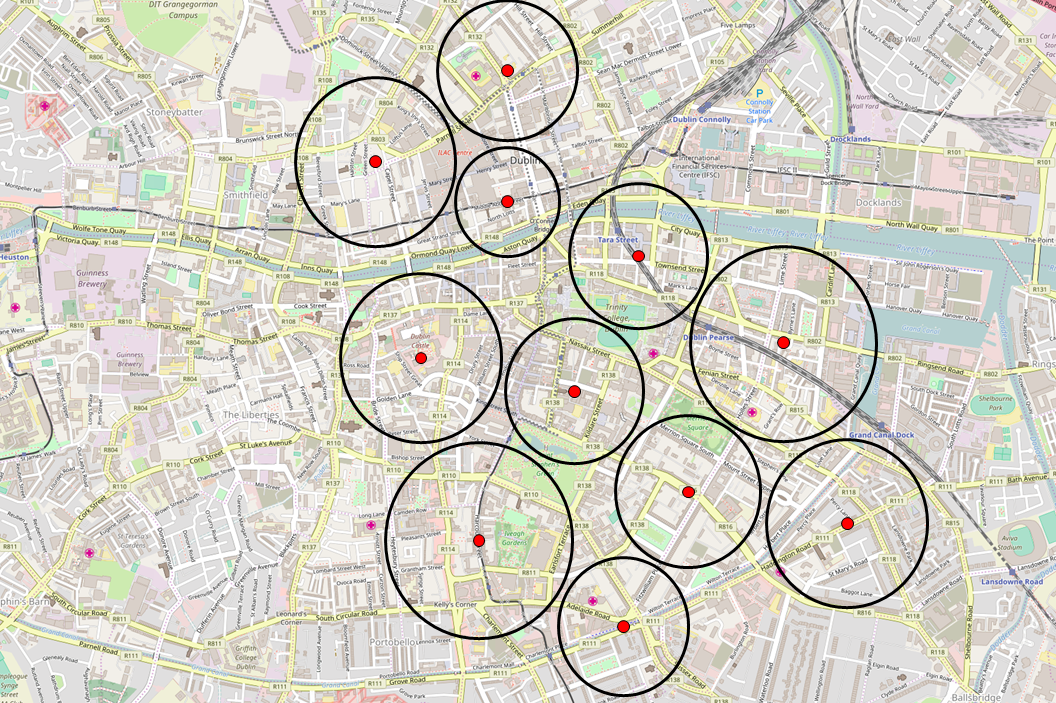
\includegraphics[width=\textwidth]{./Images/DESTINATIONSECTORSINITIAL.png}
    \caption{Destination Sectors}
    \label{fig:destination_sectors_initial}
\end{figure}

11 destination sectors are defined. Each represented by a red dot within the black circles in figure \ref{fig:destination_sectors_initial}. The black circles represent the coverage of each sector. After the vehicle has randomly chosen one of the 11 destinations, the list of all known parking areas is iterated through to find the closest parking areas to the vehicles' destination. Whether a vehicle seeks an on-street parking location or in a parking lot is defined beforehand as mentioned in the beginning of section \ref{ssec:vehicle_init}

However, this method of choosing the closest parking areas proved too deterministic. A vehicle choosing one of the red dots as seen in figure \ref{fig:destination_sectors_initial} would result in choosing identical closest parking areas for each vehicle travelling to that sector. Thus, a second pass is introduced to provide a more granular final destination allocator.

\paragraph{Granular Final Destination}
A vehicle assignment of a final destination from a finite list proved to be too deterministic. By picking a sector, the returned results for the closest parking areas within that sector will be identical to another vehicles' who chose that sector. Thus, a second pass is introduced to allow vehicle set a final destination that within the bounds of the destination sector that was initially chosen. 

\begin{figure}[H]
    \centering
    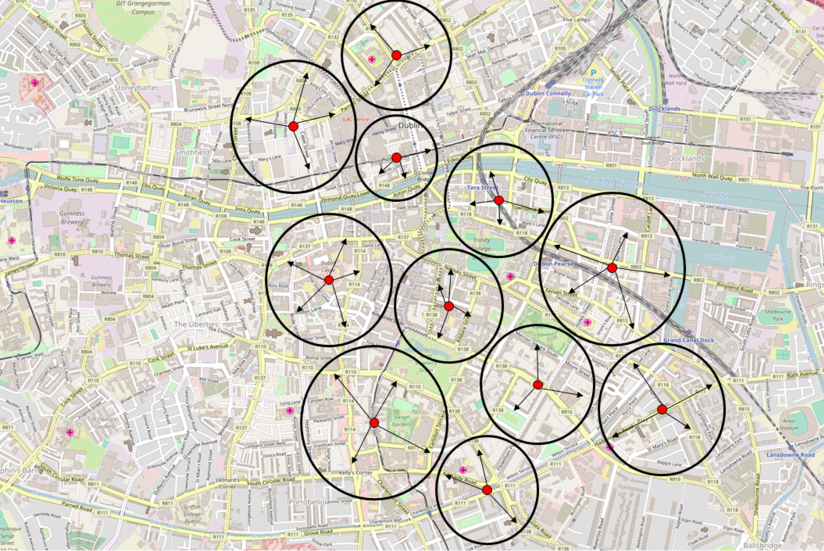
\includegraphics[width=\textwidth]{./Images/DESTINATIONSECTORS.png}
    \caption{Granular Destinations}
    \label{fig:destination_sectors}
\end{figure}

Figure \ref{fig:destination_sectors} illustrates an example of the granular destinations that vehicles could discover. All granular destinations are checked whether they lie within the bounds of the sectors.

\subsubsection{Finding Closest Parking Areas}
After a final destination for the vehicle is determined, a list of the closest parking areas relative to the vehicles' destination must be found. The process is as follows: 

\begin{enumerate}
    \item Acknowledge if the vehicle is destined for an on-street parking space or a parking lot.
    \item Using the distance formula, calculate the distances to all parking areas from the vehicles' final destination.
    \item When calculating the distances between the parking areas and the destination, query the vehicles' local copy of parking space availability for parking areas greater than 95\% full.
    \item If the parking areas are greater than 95\% full, it is not likely that they will arrive at that location and find a vacant parking space. Thus, these parking areas are discarded and not included in the resultant list.
    \item Store the parking locations that are less than 95\% full in a list.
    \item Sort the list by ascending order, so that the closest parking area is at the start of the list.
    \item Trim the list and return the first 10 parking areas.
    \item The vehicle is now able to traverse through a list of the closest parking areas relative to their final destination. This resultant list also factors in the knowledge of parking space vacancy rates of the parking areas.
\end{enumerate}

At this point, the vehicle is able to plan its route towards the closest parking area to their destination. Upon arrival, the vehicle parks the vehicle, increments its local table of parking spaces and broadcasts this update to all vehicles within its vicinity. If the parking area is full upon arrival, the vehicle re-routes to the next closest parking area on their list.

\subsection{At Every Time Step} \label{ssec:time_step}
This section explains what occurs at every time step of the simulation. Each vehicle does the following at every time step:
\begin{enumerate}
    \item A vehicle checks if they have arrived at their destined parking location. This is done simply by checking that the road that they are currently on equals to their final destinations' road identifier. If the vehicle has arrived at their final destination, then the parking space of their local parking tracker is incremented. An update message is broadcasted to other vehicles in their vicinity. The simulation time of this update is also included in this message so that on receipt, other vehicles may update their own local copies if their local copies are outdated.
    \item If they are not parked, then a message containing information regarding parking space availability is sent out. More specifically, this message contains their local parking area availability data as well as the simulation time on which it was updated. When a vehicle receives a message, it inspects the messages last updated time and updates its own local copy of parking space availabilities accordingly.
    \item A table for parked vehicles is checked. A detailed explanation of this is in section \ref{ssec:parking}.
\end{enumerate}

This concludes the explanation of the occurrences at every time step.

\subsection{Parking Duration} \label{ssec:parking}
An small issue was discovered during the implementation phase of the simulation. SUMO removes the vehicle from the simulation when the vehicle has reached the end of its route. In other terms, the vehicles are taken out of the simulation upon reaching its final destination. This became an issue as vehicles would take up the parking space indefinitely.

The solution involves keeping a list of the parking areas that the vehicles are parked, as well as the parking duration of the vehicle. At every time step, the list is checked for vehicles that have stayed for the parking duration time. When a parking duration is up, a vehicle is inserted into the simulation in the location that the previous vehicle was removed. The vehicle waits for an update of parking space availability from other vehicles. Once it receives an updated version of the parking space availabilities, the vehicle decrements its own parking spot from its own local copy and broadcasts the message to vehicles within the vicinity.

\subsection{Exit}
Vehicles are destined to exit after their parking duration is up. An exit road is chosen randomly from a finite list. This is to simulate traffic heading outbounds as well as notifying vehicles in their vicinity that the parking space is now vacant.